A natural question to ask is whether improved shared control performance can be achieved by further adapting parameters $W(\epsilon_i^\star)$ and ${W}_N(\epsilon_i^\star)$, which have a clear and direct relationship with the zone NMPC behavior -- assigning smaller values to the part corresponding to the automatic controller in $W(\epsilon_i^\star)$ and ${W}_N(\epsilon_i^\star)$, and bigger values to the part corresponding to the human inputs, will prioritize the human actions over the automatic controller, and \textit{vice versa}. We implement this idea by designing two adaptation criteria that are capable of achieving an enhanced performance in terms of sharing the control between the human operator and the automatic controller, reducing the risk of crashes. To that end, we first introduce some necessary definitions for both adaptation criteria. 

\textcolor{red}{AF: here, or actually before, in the problem setting, we need to make it clear that the main tasks consists in following a position trajectory. Also we need to make clear that going to far from the planned position is dangerous because the robot could collide with the obstacles. This is also why we focus on the position error in order to decide the mixing.}

\begin{definition}(Predicted Euclidean Distance). Let us define the distance function $\epsilon \vcentcolon \mathbb{R}^3 \rightarrow \mathbb{R}$ for an arbitrary point $p \in \mathbb{R}^3$ with respect to a reference point $p^r \in \mathbb{R}^3$ as
\begin{equation*}
	\epsilon = \|p^r-p\|_2.
\end{equation*}
	Let us then consider $p^\star_i \vcentcolon = \{p_0^\star, \dots, p_N^\star\}$ to be the optimal, predicted positions of the robot from the solution of $(\mathbf{NLP}_1)$. Suppose $\epsilon_i^\star(p) = \epsilon_i^\star$. Thus, the predicted Euclidean distance (PED) is 
	\begin{equation}
		\epsilon_i^\star = \|p_i^r-p_i^\star \|_2, \,\,\,\,\,\,\,\,\,\,\,\, i = 0, \dots, N,\label{eq:ped}%
	\end{equation}
	where $p_i^r$ is the reference trajectory of the robot.
\end{definition}

\textcolor{red}{AF: instead of just 'predicted' I would call this the 'human-off' distance, or something similar. Basically this is the distance that one would have if the human is taken completely out of the loop.}

\begin{definition}(Admissible Euclidean Distance). Consider $a \in \mathbb{R}^3$ as the maximum admissible error, in meters, with respect to the instantaneous position of the robot. We can define the admissible Euclidean distance (AED) such as:
\begin{equation}
	\epsilon_{a} = \|(p_0^r+a)-p_0^r\|_2.\label{eq:aed}%
\end{equation}

\textcolor{red}{AF: isn't this just $\|a\|_2$?}

The AED is a fixed offset along the entire trajectory, thereby one can choose any point in the reference to calculate its value, e.g. the point at stage $N=0$ was chosen \textcolor{red}{AF: isn't N the number of prediction steps?}.
\end{definition}

The zone NMPC penalizes PED excursions from a carefully designed target zone with lower and upper bounds $\check{\epsilon}$ and $\Hat{\epsilon}$, respectively. \textcolor{red}{AF: why to put a lower bound? isn't an error equal to $0$ the perfect case that we aim to?}At each time step, a zone-excursion function assigns the values of $W(\epsilon_i^\star)$ and ${W}_N(\epsilon_i^\star)$ based on an adaptation criterion that determines who, between the human and the robot, must have control authority at the moment. \textcolor{red}{AF: rather: how the control authority should be distributed among the human and the fully automatic controller.} To implement this principle, we regard two adaptation criteria and their respective zone-excursion functions: 
\begin{figure}
	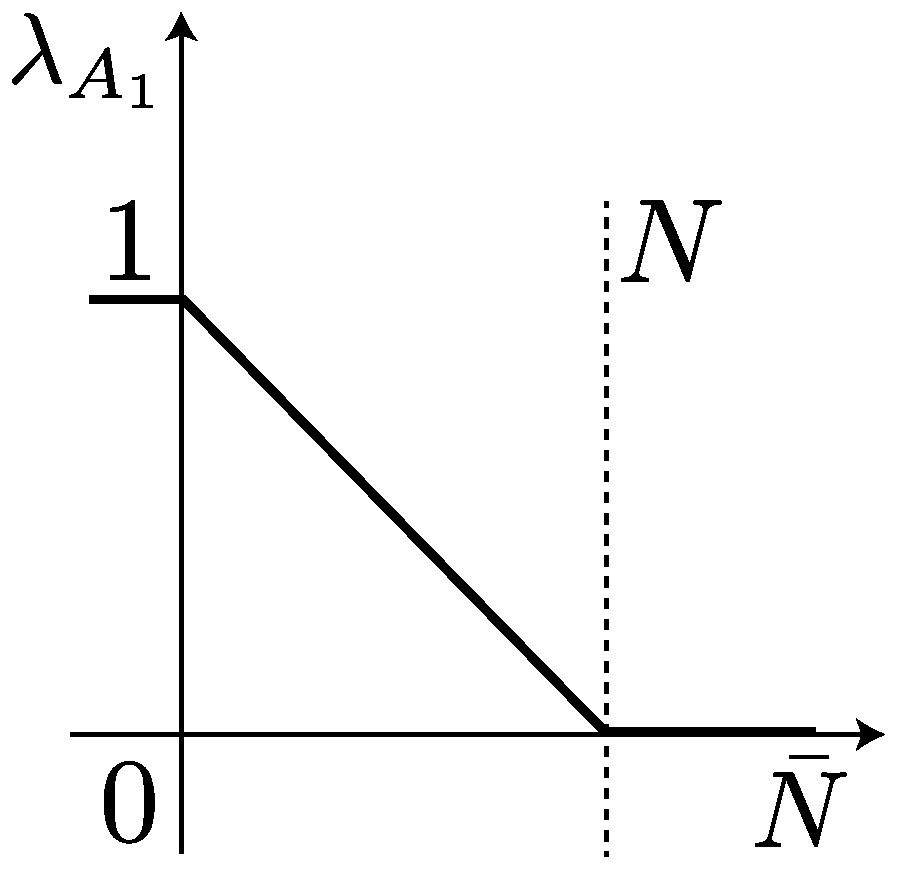
\includegraphics[width=0.40\textwidth]{figure/basic_function_a1}\hfill
	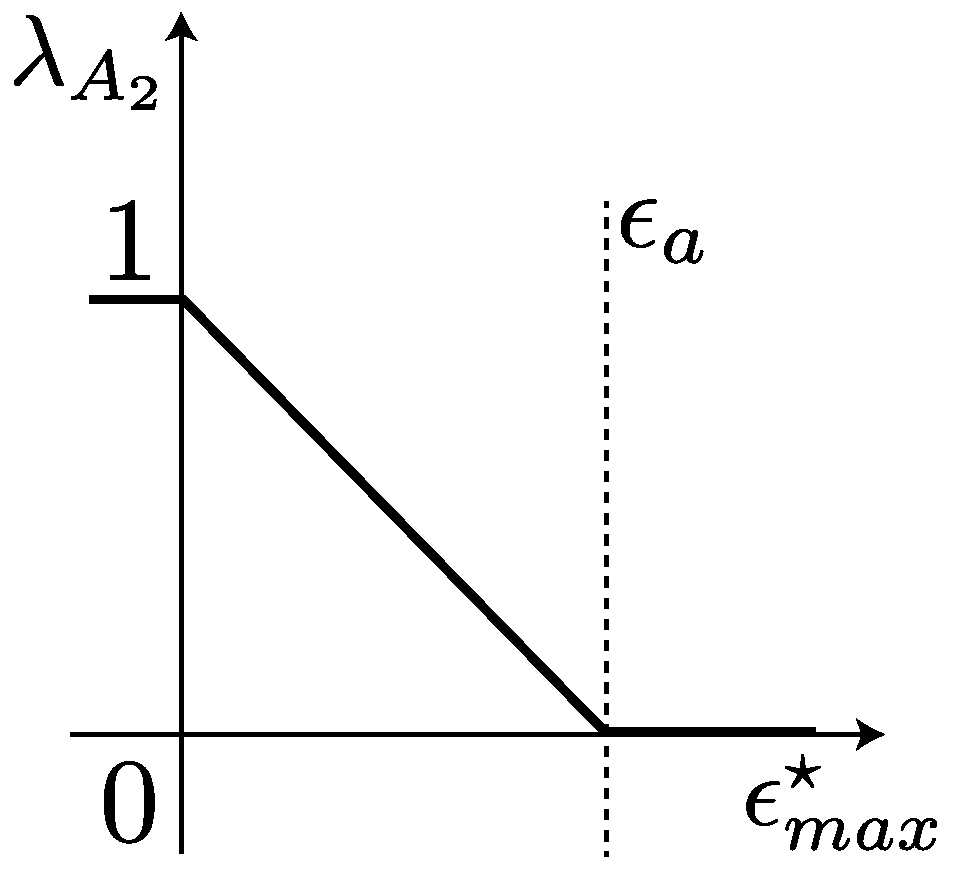
\includegraphics[width=0.43\textwidth]{figure/basic_function_a2}
	\caption{An illustration of the zone-excursion functions defined in \eqref{eq:lambda1} and \eqref{eq:lambda2} for adaptation criteria $(A_1)$ and $(A_2)$, respectively.}\label{fig:zone_functions}%
\end{figure}
\begin{enumerate}[label=(\subscript{A}{{\arabic*}}),leftmargin=40pt]
	\item 	 \textit{settling stage}: given a horizon with $N$ stages, , we select the last stage for which $\epsilon^\star_i \in [\check{\epsilon},\Hat{\epsilon}]$. \textcolor{red}{AF: define this number more formally, assuming that in the last stage the position is within the bounds then it is the minimum $i$ such that the position is in the bounds for $i$ all all the subsequent stages. Otherwise it is just $N$}.
	\textcolor{red}{AF: say that this number represents the 'time' that it would take for the fully automatic controller to bring back the position error within the bound}. 
	This stage is henceforth termed ``active shooting node", $\Bar{N}$ 	\textcolor{red}{AF I would rather call it the 'recovery time' or 'recovery stage'}. The zone-excursion function $\lambda_{A_1} \vcentcolon \mathbb{W} \rightarrow \mathbb{R}$ is defined as:
		\begin{equation}\label{eq:lambda1}%
			\lambda_{A_1} \vcentcolon = \{ \Bar{N} \vcentcolon (N-\Bar{N})/N \in [0,1] \}.
		\end{equation}
	\item \textit{maximum PED in the horizon}: given a horizon with $N$ stages, we select the maximum PED within the horizon, $\epsilon^\star_{max}$, and apply the zone-excursion function $\lambda_{A_2} \vcentcolon \mathbb{R} \rightarrow \mathbb{R}$ characterized as:
		\begin{equation}\label{eq:lambda2}%
			\lambda_{A_2} \vcentcolon = \{\epsilon^\star_{max} \vcentcolon (\epsilon_a-\epsilon^\star_{max})/\epsilon_a \in [0,1] \}.
		\end{equation}
\end{enumerate}

Moreover, assume that $W_R \in \mathbb{R}^{n_{\xi} \times n_{\xi}}, W_H \in \mathbb{R}^{n_{\nu} \times n_{\nu}}$ and $W_C \in \mathbb{R}^{n_u \times n_u}$ are the weight matrices analogous, respectively, to the contribution of the robot, human, and control input in the cost function of $(\mathbf{NLP}_2)$. 
	\textcolor{red}{AF: the control inputs seem not appear in the cost function.}
These matrices contain the initial setting over which the zone-excursion functions modulate the control authority. Thus, we denote the structure of $W(\epsilon_i^\star)$ and ${W}_N(\epsilon_i^\star)$ for both adaptation criteria\footnote{where the underscript $\bullet$ is a wildcard that specifies the zone-excursion function used for building $W(\epsilon_i^\star)$ and ${W}_N(\epsilon_i^\star)$.} as being:

\begin{eqnarray}
\begin{aligned}
	W(\epsilon_i^\star) & =  \text{blkdiag}((1-\lambda_{\bullet})\cdot W_R, \lambda_{\bullet} \cdot W_H, \lambda_{\bullet} \cdot W_C)\\
	{W}_N(\epsilon_i^\star) & = \text{blkdiag}((1-\lambda_{\bullet})\cdot W_R, \lambda_{\bullet} \cdot W_H).\label{eq:weight_matrices}
\end{aligned}
\end{eqnarray}
An illustration of each zone-excursion function is provided in Fig. \ref{fig:zone_functions}.